\chapter{Labs Overview}


\section{Performed Labs}
  As part of this experience, I had a variety of hands-on labs for which I am grateful. The following are some of the practical learning experiences I've had.
\begin{itemize}
  \item Connect to the company's internal repository hoster, to which I contributed code, documentation, and scripts.
  \item Implemented cloud service using AWS portal, AWS CLI, and other third-party applications.
  \item Performed  with CI/CD pipelines using HARNESSIO.
  \item Work on Backend tasks such as database, APIs, and queries.
  \item Deep dive networking concepts and DNS, Firewall, and VPN gateway configuration
  \item In addition to networking, I've worked in cybersecurity, including sign-up encryption and secret management.
   
  

\end{itemize}
Because I was using the internal company computer, it's nearly impossible to include all of the labs I've had there. So I'll include some of what I've had below, and you can also look around my blog for more technical/lab documentation.
\section{Internal Contribution}

Linedata NavQuest is distributed through 7 internal repositories, both locally and in the cloud (GitHub). As part of my DevOps tasks, I worked on build automation.\newline
I had an added value to the Powershell, improve the build with CSharp, and push the build to TeamCity, the company's continuous integration tool.\newline


\begin{itemize}
  \item Contribution to the product's total of seven internal repositories: Docs, Scripts, Code, Configs.
  \item Managing the continuous integration process: Teamcity, GitHub, Docker, Powershell and terraform.
  \item In addition to using Harness, Ansible, and AWS to test the CD along with spending time documenting.

\end{itemize}

\subsection{GitHub Repository}

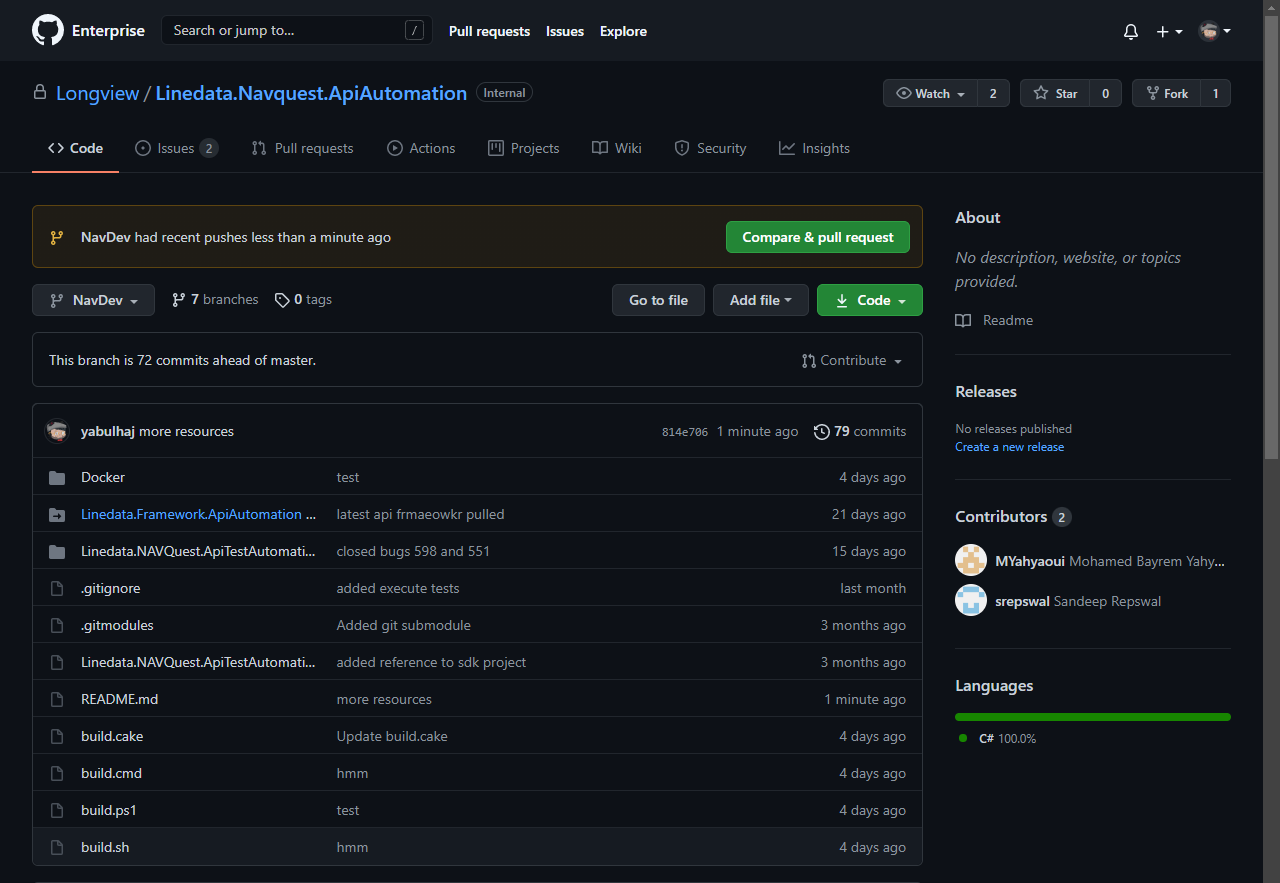
\includegraphics[width=.9\columnwidth]{Rapport ISTIC/p1.png}\\
\newline
\textbf{Part of the documentation:}\newline

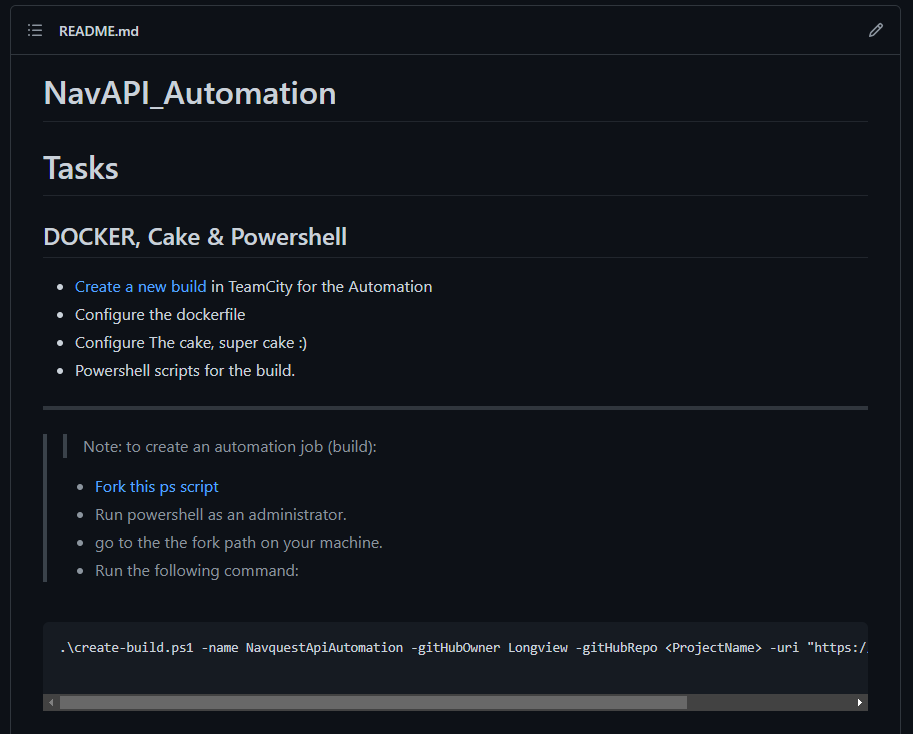
\includegraphics[width=.9\columnwidth]{Rapport ISTIC/p2.png}\\

\subsection{HARNESSIO}
Rather than real scripting, Harness uses a model to define your goals. Although you can use YAML within Harness, you do not need to write a script for the pipeline. The real advantage here is that you can simply select these steps, stages, and every component required for the configuration file using a user-friendly interface. I worked with colleagues to script the pipeline using the UI with HARNESS.\newline

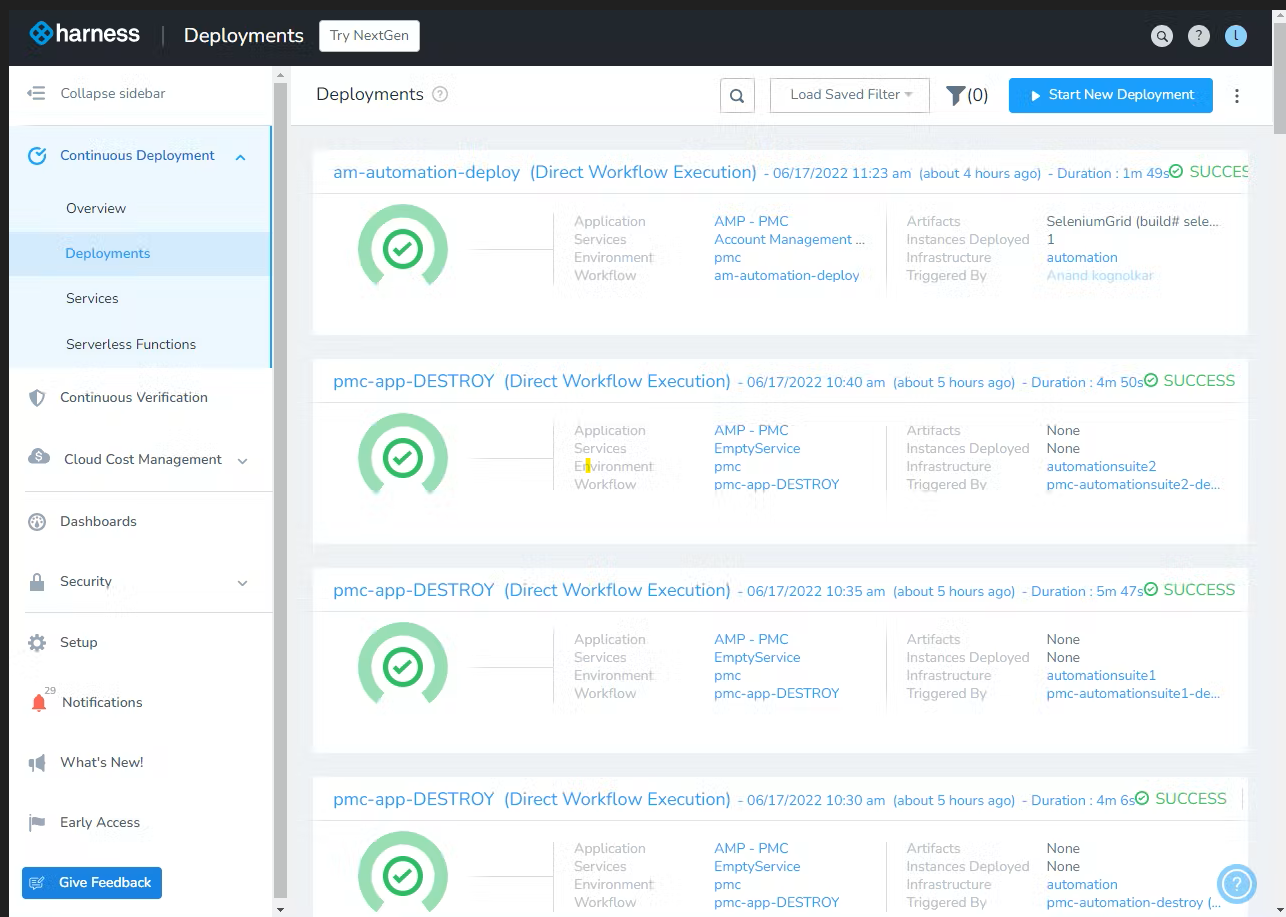
\includegraphics[width=1\columnwidth]{Rapport ISTIC/har.png}\\

\subsection{KUBERENETES}

Linedata is built entirely on the powerful container orchestration tool kubernetes. As earlier described, containers and docker are critical components. K8s simply make it easier to manage a large number of them. I spent a considerable amount of time managing the clusters, which included the pods that ran the containerized apps.\newline

Some of the tasks were as followed:
\begin{itemize}
  \item Install and Set Up kubectl on Windows.
  \item Certificate Management with kubeadm.
  \item Upgrading Windows nodes.
  \item Migrate Docker Engine nodes from dockershim to cri-dockerd.

\end{itemize}